%%%%%%%%%%%%%%%%%%%%%%%%%%%%%%%%%%%%%%%%%
% University Assignment Title Page 
% LaTeX Template
% Version 1.0 (27/12/12)
%
% This template has been downloaded from:
% http://www.LaTeXTemplates.com
%
% Original author:
% WikiBooks (http://en.wikibooks.org/wiki/LaTeX/Title_Creation)
%
% License:
% CC BY-NC-SA 3.0 (http://creativecommons.org/licenses/by-nc-sa/3.0/)
% 
% Instructions for using this template:
% This title page is capable of being compiled as is. This is not useful for 
% including it in another document. To do this, you have two options: 
%
% 1) Copy/paste everything between \begin{document} and \end{document} 
% starting at \begin{titlepage} and paste this into another LaTeX file where you 
% want your title page.
% OR
% 2) Remove everything outside the \begin{titlepage} and \end{titlepage} and 
% move this file to the same directory as the LaTeX file you wish to add it to. 
% Then add \input{./title_page_1.tex} to your LaTeX file where you want your
% title page.
%
% template taken from https://www.overleaf.com/latex/examples/title-page-with-logo/hrskypjpkrpd#.WDXHQKIrLdc
%%%%%%%%%%%%%%%%%%%%%%%%%%%%%%%%%%%%%%%%%
%\title{Title page with logo}
%----------------------------------------------------------------------------------------
%   PACKAGES AND OTHER DOCUMENT CONFIGURATIONS
%----------------------------------------------------------------------------------------

\documentclass[12pt]{article}
\usepackage[english]{babel}
\usepackage[utf8x]{inputenc}
\usepackage{algpseudocode}
\usepackage{algorithm}
\usepackage{algorithmicx}
\usepackage{amsmath}
\usepackage{courier}
\usepackage{graphicx}
\usepackage{hyperref}
\usepackage{listings}
\usepackage{url}
\usepackage[colorinlistoftodos]{todonotes}

\begin{document}

\begin{titlepage}

\newcommand{\HRule}{\rule{\linewidth}{0.5mm}} % Defines a new command for the horizontal lines, change thickness here

\center % Center everything on the page
 
%----------------------------------------------------------------------------------------
%   HEADING SECTIONS
%----------------------------------------------------------------------------------------

\textsc{\LARGE The University of Texas at Austin}\\[1.5cm] % Name of your university/college
\textsc{\Large Distributed Systems}\\[0.5cm] % Major heading such as course name
\textsc{\large Software Engineering - Option III}\\[0.5cm] % Minor heading such as course title

%----------------------------------------------------------------------------------------
%   TITLE SECTION
%----------------------------------------------------------------------------------------

\HRule \\[0.4cm]
{ \huge \bfseries Fleeing Paxos by Raft}\\[0.4cm] % Title of your document
\HRule \\[1.5cm]
 
%----------------------------------------------------------------------------------------
%   AUTHOR SECTION
%----------------------------------------------------------------------------------------

\begin{minipage}{0.4\textwidth}
\begin{flushleft} \large
\emph{Authors:}\\
Howie \textsc{Benefiel}\\
Patrick \textsc{Sigourney} % Your name
\end{flushleft}
\end{minipage}
~
\begin{minipage}{0.4\textwidth}
\begin{flushright} \large
\emph{Professor:} \\
Dr. Vijay \textsc{Garg} % Supervisor's Name
\end{flushright}
\end{minipage}\\[2cm]

% If you don't want a supervisor, uncomment the two lines below and remove the section above
%\Large \emph{Author:}\\
%John \textsc{Smith}\\[3cm] % Your name

%----------------------------------------------------------------------------------------
%   DATE SECTION
%----------------------------------------------------------------------------------------

{\large \today}\\[2cm] % Date, change the \today to a set date if you want to be precise

%----------------------------------------------------------------------------------------
%   LOGO SECTION
%----------------------------------------------------------------------------------------


\includegraphics{logo.png}\\[1cm] % Include a department/university logo - this will require the graphicx package
 
%----------------------------------------------------------------------------------------

\vfill % Fill the rest of the page with whitespace

\end{titlepage}


\begin{abstract}
    Paxos has been the industry-standard protocol for implementing distributed consensus for the past 25 years.
    Though the basics of single-decree consensus are easily enough grokked, delving into why it works, forming a replicated log or implementing membership changes is fraught with unproven ambiguity.
    Raft was designed with a singular design goal, understandability.
    To achieve this goal of optimizing for understandability, the authors employed two techniques, problem decomposition and minimization of state space.
    For this paper, we examined and implemented their protocol.
    We found their protocol performed as well as they claimed and it was much easier to fundamentally grok than Paxos.
\end{abstract}

\section{Introduction}

The primary focus of distributed consensus is to take an unreliable machine and replicate it so that it becomes a cluster of individually unreliable but collectively reliable machines.
The most studied model for this is the replicated state machine model.
In this model, each machine has some internal state which can be changed by external stimulus.
Perhaps obviously, the state of these state machines should be replicated by all the machines in the cluster.
At a high level, the duty of a distributed consensus protocol is to ensure the state stays consistent across all the machines in the cluster.

The core data structure in a practical consensus algorithm, and indeed Raft, is the replicated log.
The replicated log contains all the commands that have been run against the cluster.
If a machine were to start at the beginning of the log and execute each command in its log in order that machine should arrive at a state consistent with other machines in the cluster.
At a more practical level, a distributed consensus protocol will keep these replicated logs consistent across the cluster.

The FLP Impossibility Proof states that an asynchronous distributed system can not tolerate failure while satifying agreement, validity and termination. \cite{flp-theorem}
So consensus algorithms, including Raft, generally satisfy:
\begin{enumerate}
    \item \textit{Safety} They always return a correct result.
    If a client randomly queries any server for the state of the system, the result should be the same regardless of which machine was queried.
    \item \textit{Availability} If a majority of the servers are available, the system, as a whole should be available.
    \item \textit{Time Invariance} The system should not depend on the physical timing of events.
    \item \textit{Quorum Limited} The response to the client should be returned once quorum is reached, not when all machines have responded.
\end{enumerate}

Paxos, the leading distributed consensus algorithm thusfar, satisfies these properties, but its original incantation only arrived at consensus on a single value. \cite{long-form-paxos}
Practical systems need to build a replicated log which is an extension of the original Paxos protocol.
This extension is one symptom of a larger problem with Paxos where extensions are needed to build practical systems with these extensions not being formally studied.
Furthermore, the single-decree Paxos protocol is challenging enough in itself to understand, so extensions are incredibly hard to fully grok.

Since Paxos is poorly suited for building practical systems due to its complexity, the authors of Raft designed their protocol for understandability.
This is obviously a unique goal as compared to most other CS papers, where the goal is to improve some time, memory, or message complexity.

The authors worked toward this goal using two techniques: decomposing the primary problem, distributed consensus, into independent sub-problems and minimizing the state space of the algorithm.

In this work, we examine the Raft algorithm, implement it and examine its performance

\section{Algorithm Overview}

Whereas Paxos shares a solution detail among multiple sub-problems, Raft targets a few sub-problems independent of one another.
Before we discuss how Paxos solves these sub-problems, there are a few structures which we need to explain.

\subsection{Structures}
First, there is the concept of a \textit{term}.
A term is a subset of the system's execution which begins with an election of a leader.
A term concludes when the elected leader is not longer able to send messages to the other members of the cluster, usually due to the leader process failing, and a new election is started by the remaining cluster members.
In exceptional circumstances, a term can end with no leader being elected due to a draw in voting, which results in a new term and new election being initiated.

The second structure described by Raft is the replicated log.
The replicated log, as touched on above, is a list with each entry containing the command received from a client and the term number in which the command was received. Each entry is stored at a unique, incremented index location within the log.
An example of the replicated log is shown below in Fig.~\ref{fig:replicatedlog}.

\begin{figure}
    \centering{}
    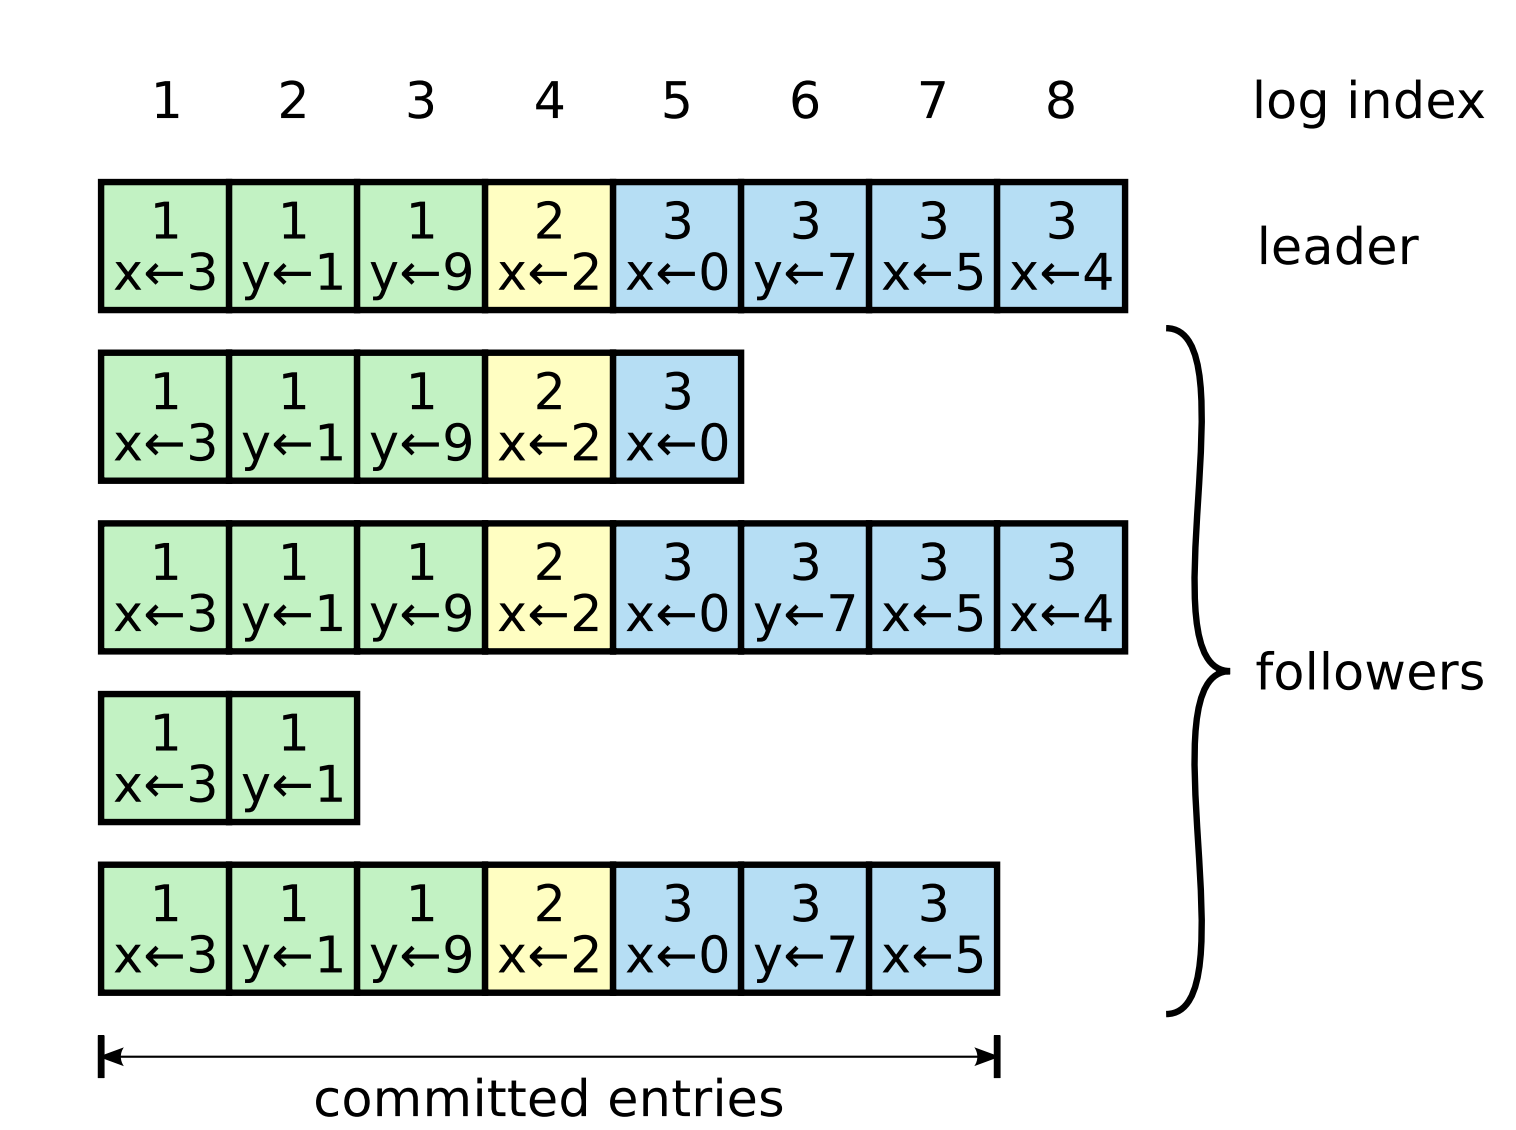
\includegraphics[width=0.75\textwidth]{replicatedlog.png}
    \caption{\label{fig:replicatedlog}Above is an example of a replicated log. The top number and the color represent the term and the index of each entry is at the top.}
\end{figure}

Raft also uses two RPC messages, both having well defined schema.
The purpose and implications of each will be discussed later in the paper but they will be introduced here.
First, the \texttt{RequestVote} RPC is used by a candidate who has initiated an election and is sent to all other servers to request their vote for leader in the new term.

Second, the \texttt{AppendEntries} RPC is used for two purposes:
Primarily it is used by the leader to replicate its logs among the followers.
An empty \texttt{AppendEntries} RPC is also used as a heartbeat mechanism by the leader, to notify the followers that the leader is still alive and in control.
When a follower's logs are determined to be inconsistent with the leader's logs, the \texttt{AppendEntries} RPC is used to rewind the inconsistent follower's state and bring the follower into a state consistent with the leader.
We have found that this RPC is somewhat overloaded and it would help understandability to decompose this RPC into a \texttt{HandleLogs} RPC and a \texttt{Heartbeat} RPC.

\subsection{Subproblems}

\subsubsection{Leader Election}

Using these data structures, the first of the sub-problems which Raft solves is leader election.
Like Paxos and unlike some other consensus protocols such as Egalitarian Paxos \cite{e-paxos}, Raft elects a leader.
In the Raft model, a machine can exist in one of three states: leader, candidate, or follower.
A machine initial starts in a follower state.  Every follower maintains a countdown timer with a random value within a preset range, the \texttt{election\_interval}.  This randomizing ensures that the timers expire at staggered intervals rather than simultanously.  When a follower receives an \texttt{AppendEntries} RPC (whether a log update or a heartbeat message), the timer is reset.  If the timer expires, the follower will increment its term, convert to a candidate, and send \texttt{RequestVote} RPCs to all other machines in the cluster.

That candidate then waits to receive votes from a majority of machines for that term.  This rule mandates that a Raft cluster can only withstand the loss of 1/2 n - 1 members and still persist.  If greater than half the members fail, none of the remaining machines will be able to achieve an election majority and a new leader cannot be elected.
 
While holding an election, if a candidate receives an \texttt{AppendEntries} RPC with a term greater than or equal to the candidate's term, the candidate knows there is a legitimate leader in the system and reverts itself back to a follower.
If an \texttt{AppendEntries} RPC is received with a term less than the recipient's, the recipient will reply back to the sender with current term value which will result in the sender (who believes himself a leader) updating his term value and setting himself as a follower.
Once a candidate receives a majority of votes from the cluster members, it has been elected leader for the term and will begin sending heartbeat \texttt{AppendEntries} RPC messages to the other members which will reset their election clocks and prevent an election from starting.

\subsubsection{Log Replication}

The second sub-problem Raft solves is log replication.
This problem is markedly more complicated.

To more easily handle this problem, Raft defines two properties for the logs:
First, two machines with log entries at the same index with the same term will contain the same command.
This property allows us to couple ordering to the state of the system.
Building on the first property, two machines containing log entries with the same index and term implies all previous log entries are identical between the machines.
By defining these invariants, Raft simplifies the safety of the system.

The happy path case of log replication is when a leader receives a request from a client, the leader appends the request to its log, sends the \texttt{AppendEntries} RPC and the followers append the log entry to their logs.
The last step of the process is the leader marking the log entry as committed once the leader receives replies of \texttt{success} to an \texttt{AppendEntries} RPC from a majority of the members of the cluster, the leader marks the entry as committed and the entry can then be applied to the state machine with the knowledge that a majority of the other cluster members will also apply the entry.

The unhappy path is when there are a series of leader and follower crashes.
In this case, the system needs a way of rectifying the competing logs into a consistent state.
The system accomplishes this by overloading the \texttt{AppendEntries} RPC.
Whenever a leader sends an \texttt{AppendEntries} RPC, it includes \texttt{prevLogIndex} and \texttt{prevLogTerm} values which contains the index and term of the leader's previous committed log entry.
If a follower receives this \texttt{AppendEntries} RPC and the \texttt{prevLogIndex} and \texttt{prevLogTerm} do not match the follower's log values, the follower will return false.
The leader will then rewind and send step back through the log, sending messages with earlier log entries until the follower finds the last log entry which matches the leader's log.  At this point, the leader will play forward through its log to bring the follower's log up to date.
Using this mechanism, the current leader can rectify inconsistencies in the follower's logs and ensure consistency across the cluster.


\subsubsection{Safety}

The above properties are not sufficient to ensure safety.
For instance, imagine a machine has been down for some time and then it is elected leader.
It would overwrite committed log entries which would result in machines being in different states.
Raft employs two mechanisms by which it ensures safety.

First, when a candidate initiates an election, it sends the term of its last committed entry.
If a follower receives that \texttt{RequestVote} RPC and the follower's term is greater than the candidate's, the follower will refuse to vote for that candidate.
Since a majority of the cluster had to have had a value for it to be committed, that candidate with a stale term will not win.

Second, it is possible that an entry had been sent to a majority of servers, but the leader crashed before it can send the heartbeat which would cause the entries to be committed.
In this case, Raft has two options here.
One solution is to develop some protocol to count replicas for previous terms and send commits for those terms.
Another is to have the current leader only commit for its term.
Once there is a commit at the ``head'' of the log, all previous entries can be assumed to be committed.
The first method has some peculiar edge conditions, but the second could slow progress.
Since this Raft, the authors decided on the simpler method.


\section{Implementation \& Conclusion}
Using tha paper and other online material from the authors we implemented the protocol in Java successfully.
Furthermore, we were able to implement this replicated state machine system in many fewer lines of code than previous attempts.

After this implementation, we feel Raft has accomplished its goal: to create a viable, understandable alternative consensus algorithm to Paxos which does not require having to stray from the defined algorithm in order to build a real-world implementation.  We hope the idea of simplicity and understandability in algorithmic design will take hold and other researchers will continue the trend started by Ongaro and Ousterhout with Raft.



\newpage


\bibliographystyle{plain}
\bibliography{references}



\appendix

\section{Github Code}

\href{https://github.com/psigourney/raft_consensus}{https://github.com/psigourney/raft\_consensus}

%\section{Thread-Local Example}
%\label{sec:tls}
%\lstinputlisting[language=Java, firstline=366, lastline=382]{../../java-bag/src/SwedishBag.java}
% \section{Some \LaTeX{} Examples}
% \label{sec:examples}

% \subsection{Sections}

% Use section and subse{}ction commands to organize your document. \LaTeX{} handles all the formatting and numbering automatically. Use ref and label commands for cross-references.

% \subsection{Comments}

% Comments can be added to the margins of the document using the \todo{Here's a comment in the margin!} todo command, as shown in the example on the right. You can also add inline comments too:

% \todo[inline, color=green!40]{This is an inline comment.}

% \subsection{Tables and Figures}

% Use the table and tabular commands for basic tables --- see Table~\ref{tab:widgets}, for example. You can upload a figure (JPEG, PNG or PDF) using the files menu. To include it in your document, use the includegraphics command as in the code for Figure~\ref{fig:frog} below.

% % Commands to include a figure:
% \begin{figure}
% \centering
% \includegraphics[width=0.5\textwidth]{frog.jpg}
% \caption{\label{fig:frog}This is a figure caption.}
% \end{figure}

% \begin{table}
% \centering
% \begin{tabular}{l|r}
% Item & Quantity \\\hline
% Widgets & 42 \\
% Gadgets & 13
% \end{tabular}
% \caption{\label{tab:widgets}An example table.}
% \end{table}

% \subsection{Mathematics}

% \LaTeX{} is great at typesetting mathematics. Let $X_1, X_2, \ldots, X_n$ be a sequence of independent and identically distributed random variables with $\text{E}[X_i] = \mu$ and $\text{Var}[X_i] = \sigma^2 < \infty$, and let
% $$S_n = \frac{X_1 + X_2 + \cdots + X_n}{n}
%       = \frac{1}{n}\sum_{i}^{n} X_i$$
% denote their mean. Then as $n$ approaches infinity, the random variables $\sqrt{n}(S_n - \mu)$ converge in distribution to a normal $\mathcal{N}(0, \sigma^2)$.

% \subsection{Lists}

% You can make lists with automatic numbering \dots

% \begin{enumerate}
% \item Like this,
% \item and like this.
% \end{enumerate}
% \dots or bullet points \dots
% \begin{itemize}
% \item Like this,
% \item and like this.
% \end{itemize}

% We hope you find write\LaTeX\ useful, and please let us know if you have any feedback using the help menu above.



\end{document}
